\documentclass[utf8, 11pt]{beamer}
\usepackage{verbatim}
\usepackage{color}
\usepackage{graphicx}
\usepackage{alltt}
%\usepackage{hyperref}
%\hypersetup{colorlinks=true, urlcolor=cyan}
\hypersetup{urlcolor=cyan}

\mode<presentation>
{
  \usetheme{default}
}

\usepackage[english, russian]{babel}
\usepackage{graphicx}
\usepackage{colortbl}

\newcommand{\rsb}{\cellcolor[gray]{0.85}}
\newcommand{\nam}[1]{\texttt{#1}}

\setbeamertemplate{navigation symbols}{} 

\author[ ]{Выполнили: Савенко С. А., Карташов Д. А., Аверьянов И. Н. \\ Руководитель: Кринкин К. В.}

\title[Virtual HSM]{Разработка виртуального HSM для платформы Linux}


\institute[СПбАУ]
{
  Кафедра математических и информационных технологий\\
  Санкт-Петербургский Академический университет
}

\date{ 2013 }

\subject{Talks}

\useoutertheme{infolines}
\setbeamertemplate{headline}{}

\begin{document}

\begin{frame}
  \titlepage
\end{frame}

\begin{frame}{Введение}

Криптография в приложениях:
\begin{itemize}
\item секретные данные
\item вычисления с их использованием
\item проблемы безопасности
\end{itemize}

\vspace*{\fill}

Решение:
\begin{itemize}
\item исключить попадание секретных данных на диск и/или в память компьютера
\end{itemize}

\end{frame}

\begin{frame}{Цели и задачи проекта}

\begin{block}{Цель}
Разработать решение, предоставляющее функциональность HSM в виртуальном окружении
\end{block}

\vspace*{\fill}

\begin{block}{Задачи}
\begin{itemize}
\item поиск существующих решений;
\item поиск стандартов HSM;
\item обзор приложений, использующих криптографию;
\item разработка клиентского API;
\item реализация VHSM;
\item реализация системы хранения секретных данных;
\end{itemize}
\end{block}

\end{frame}

\begin{frame}{Предварительная работа}

Существующие решения:
\begin{itemize}
\item Amazon CloudHSM:

\url{http://aws.amazon.com/cloudhsm/}
\end{itemize}

\vspace*{\fill}

Стандарты HSM:
\begin{itemize}
\item pkcs\#11:

\url{http://www.rsa.com/rsalabs/node.asp?id=2133}
\end{itemize}

\vspace*{\fill}

%\includegraphics[width=0.32\textwidth]{img1}
\begin{center}
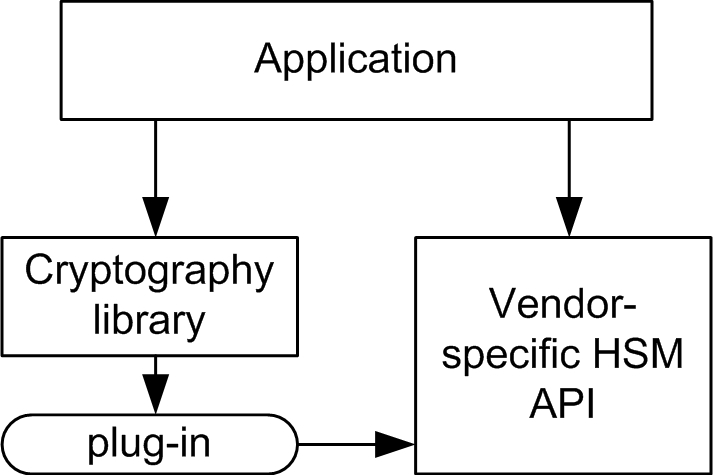
\includegraphics[scale=0.75]{img1-2}
\end{center}

\end{frame}

\begin{frame}{Архитектура решения}
\begin{center}
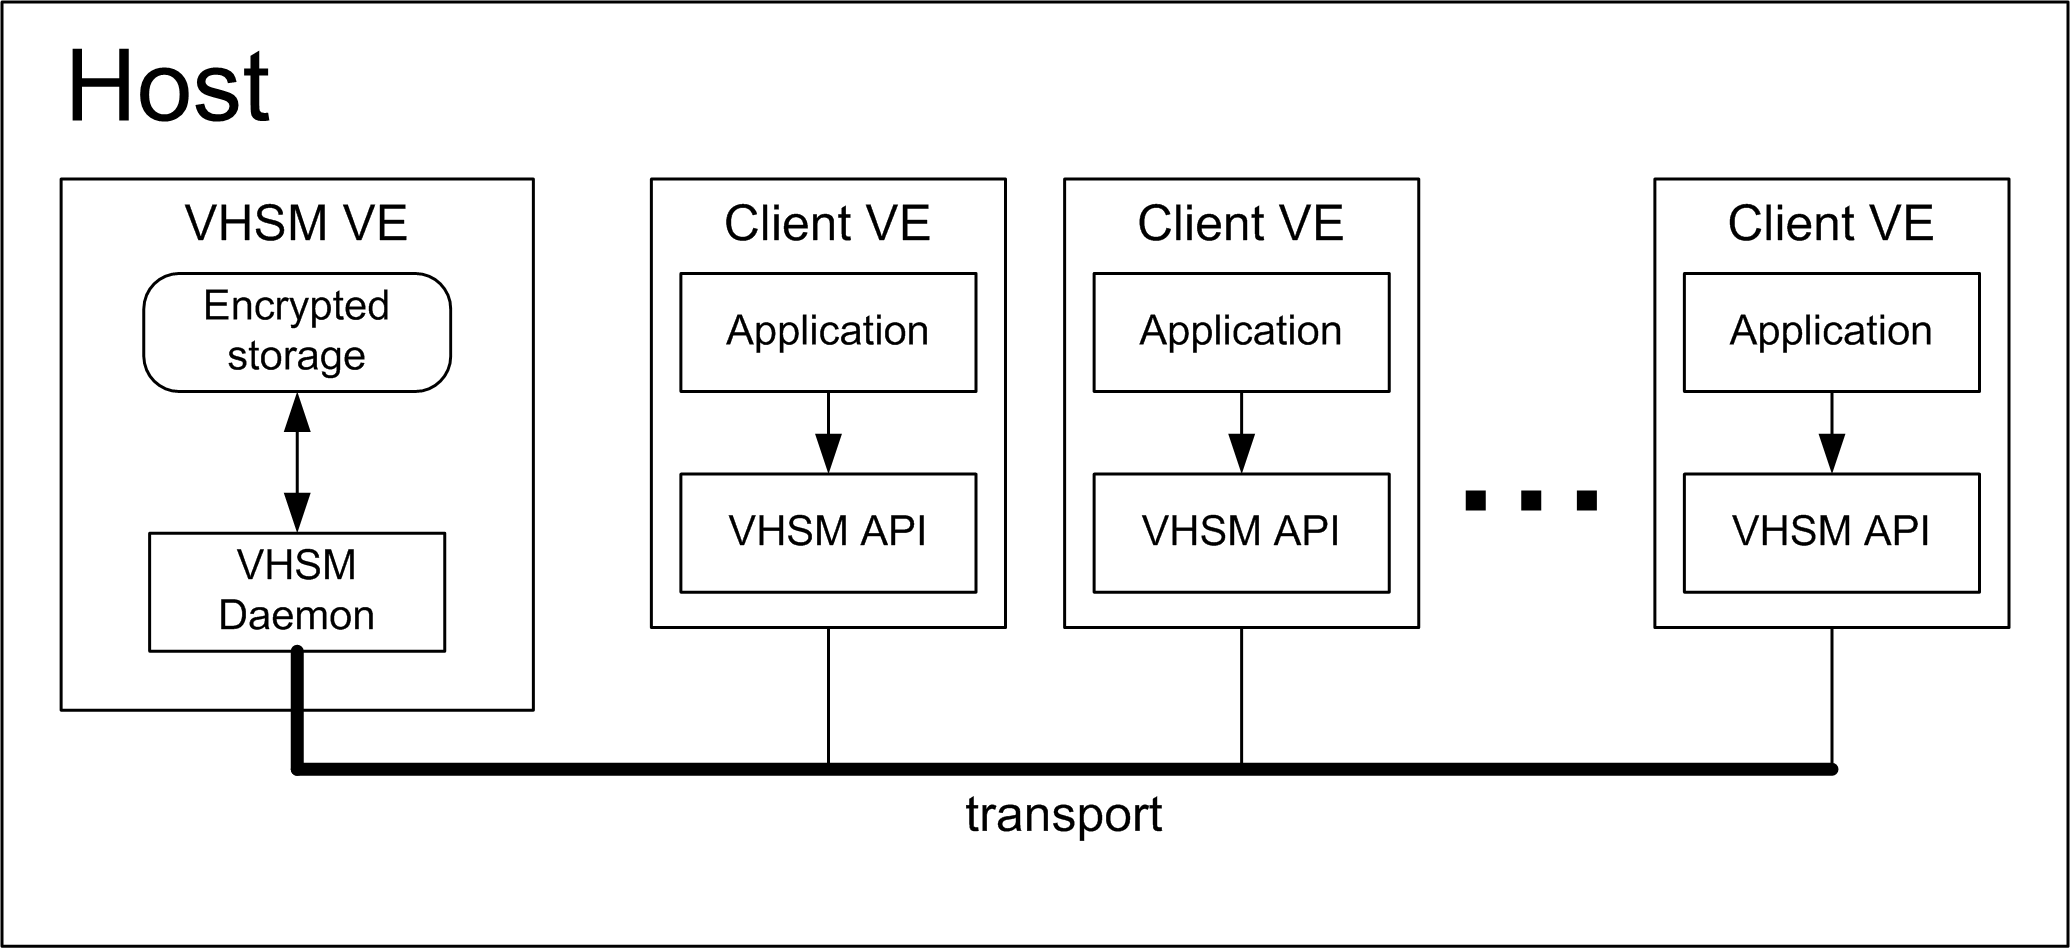
\includegraphics[width=0.95\paperwidth]{img2}
\end{center}
\end{frame}

\begin{frame}{Архитектура решения}
\begin{itemize}
\item Протокол:
	\begin{itemize}
	\item \texttt{Google protobuf}
	\end{itemize}
\item Траспорт:
	\begin{itemize}
	\item файловая система
	\end{itemize}
\item Защищенное хранилище:
	\begin{itemize}
	\item файловая система
	\item \texttt{AES}
	\end{itemize}
\item Криптография:
	\begin{itemize}
	\item \texttt{crypto++}
	\end{itemize}
\end{itemize}

\vspace*{\fill}
	
\end{frame}

\begin{frame}{Итоги}
\begin{itemize}
\item Реализован прототип:
	\begin{itemize}
		\item MAC
		\item хэш-функции
		\item управление ключами
	\end{itemize}
	
\item Изучены технологии:
	\begin{itemize}
		\item криптография
		\item protobuf
		\item OpenSSL
		\item pkcs\#11
		\item crypto++
		\item OpenVZ
		\item netlink
	\end{itemize}
	
\end{itemize}

\vspace*{\fill}

\end{frame}

\begin{frame}{Ссылки}
\begin{itemize}
\item Репозиторий проекта:

\url{https://github.com/OSLL/vhsm}

\item wiki проекта:

\url{http://osll.spb.ru/projects/vhsm/wiki}
\end{itemize}

\vspace*{\fill}

\end{frame}

\end{document}
